%% Short data paper template
%% Created by Simon Hengchen and Nilo Pedrazzini for the Journal of Open Humanities Data (https://openhumanitiesdata.metajnl.com)

\documentclass[11pt]{article}
\usepackage[english]{babel}
\usepackage[utf8]{inputenc}
\usepackage{johd}
\usepackage{ragged2e}


\begin{document}

\thispagestyle{empty}
%%%%%%%%%%   Edit the thesis title here   %%%%%%%%%%


\begin{figure}[!h]
\centering

\includegraphics{uzh_logo.pdf}\\\
\end{figure}
\vspace{1cm}

\begin{center}
\huge {Cryptocurrencies and the risk-free rate}
\end{center}
\vspace{1cm}

\begin{center}
\large \textbf{Final Project}\\
\vspace{0.5cm}
Digital Tools for Finance (L) (03SMDFOEC008)\\
Department of Banking and Finance, University of Zurich\\
Igor Pozdeev
\end{center}
\vspace{1cm}

\begin{center}
\large \textbf{Authors}\\
\vspace{0.5cm}
Jakob Pirs (XX-XXX-XX, jakob.pirs@uzh.ch)\\

Nina Erminia Cantoni (17-709-221, ninaerminia.cantoni@uzh.ch)\\

Rohit Koonireddy (XX-XXX-XX, rohit.koonireddy@bf.uzh.ch)\\

Yunxiang Guo (XX-XXX-XX, yunxiang.guo@uzh.ch)\\
\end{center}
\vspace{1cm}

\begin{center}
\large \textbf{Abstract}\\
\vspace{0.5cm}
\begin{justify}
tbd
\end{justify}
\end{center}
\vspace{1cm}


\begin{center}
\vfill{}
\par\end{center}

\begin{center}
\renewcommand{\today}{\ifcase \month \or January\or February\or March\or   April\or May \or June\or July\or August\or September\or October\or November\or  December\fi, \number \year} 

\begin{center}
\large{\today}
\end{center}
\end{center}

\pagebreak{}
\pagebreak{}


\setcounter{page}{1}
\section{Context and motivation}


The goal of this paper is to analyze the correlation between the 10 Year Treasury Yield and cryptocurrencies. The 10 Year Treasury Rate is the yield one receives for investing in US government securities with a maturity of 10 years. It is a common proxy for the risk free rate. Therefore, this paper will shed light on the influence of the risk free rate on the price of cryptocurrencies. \\

We considered 4 different cryptocurrencies, namely Bitcoin, Etherium,  XRP (Ripple) and Litecoin. As of November 2022, all four were within the 15 cryptocurrencies with the highes market capitalization (see for example Quelle 2). Furthermore we consider a cryptocurrency index called  CMC Crypto 200 Index by Solactive. The CMC Crypto 200 Index tracks the price movementes of the top 200 cryptocurrencies by market capitalization. It was launched at year end 2018 and is calculated and distributed by Solactive AG. The index is published in USD. Calculation of the index price is conducted on a daily basis. (Quelle 1)



\\

Quelle 1: https://www.solactive.com/wp-content/uploads/2019/04/Solactive-Index-Guideline-CMC200.pdf
Quelle 2: https://www.coingecko.com/


\subsection{In-text citations}
This journal uses a style based on the APA system (see \href{https://openhumanitiesdata.metajnl.com/about/submissions/#References}{here}). \\
The following are some basic citation commands in \LaTeX: \\

\noindent
\verb|\citet| $\rightarrow$ \citet{jenset&mcgil}\\
\verb|\citet| $\rightarrow$ \citet{australiashealth}\\
\verb|\citet| $\rightarrow$ \citet{shree-a}\\
\verb|\citep| $\rightarrow$ \citep{fabricius-hansen2012b}\\
\verb|\citealp| $\rightarrow$ (\citealp{eckhoff2018a})\\
\verb|\citealp| $\rightarrow$ (\citealp{eckhoff2018a}; \citealp{fabricius-hansen2012b}; \citealp{shree-a})\\

\subsubsection{Other simple functions}
To add bullet points:

\begin{itemize}
    \item Some point
    \item Another point
\end{itemize}

\noindent Or numbered points:

\begin{itemize}
    \item[1.] Some numbered point
    \item[2.] Another numbered point
\end{itemize}

\noindent This is an example of footnote\footnote{This is a footnote}. \\

\noindent This is a simple table:

\begin{table}[H]
\centering % Label your table accordingly
\caption{\label{tab1} A caption.}
\begin{tabular}{cccc}
\hline
1 & 2 & 3 & 4 \\
\hline
a & b & c & d\\
e & f & g & h\\
\hline
\end{tabular}
\end{table}

\noindent Please refer to your table using: Table \ref{tab1}.\\

\noindent To add a figure, upload the figure into the \texttt{images} folder, and then embed it:

\begin{figure}[H]
\centering
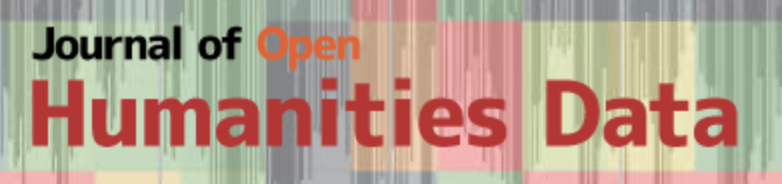
\includegraphics{images/image.jpg}
\caption{\label{fig1}JOHD's logo.}
\end{figure}

\noindent To resize the figure:

\begin{figure}[H]
\centering
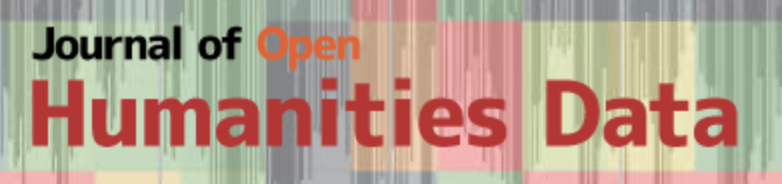
\includegraphics[width=0.2\textwidth]{images/image.jpg}
\caption{\label{fig2}JOHD's logo.}
\end{figure}

\begin{figure}[H]
\centering
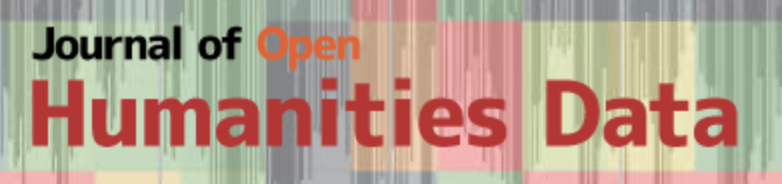
\includegraphics[width=0.8\textwidth]{images/image.jpg}
\caption{\label{fig3}JOHD's logo.}
\end{figure}

\noindent Please refer to your figures as: Figure \ref{fig1}, Figure \ref{fig2}, etc.


\section{Dataset description}
Here you can provide, if applicable, information about the dataset(s) whose creation, collection, management, access, processing or analysis have been discussed in this paper, following this schema:
\paragraph{Object name} Typically the name of the file or file set in the repository.
\paragraph{Format names and versions} E.g., ASCII, CSV, Autocad, EPS, JPEG, Excel, SQL, etc.
\paragraph{Creation dates} The start and end dates of when the data was created (YYYY-MM-DD).
\paragraph{Dataset creators} Please list anyone who helped to create the dataset (who may or may not be an author of the data paper), including their roles (using and affiliations).
\paragraph{Language} Languages used in the dataset (i.e., for variable names etc.).
\paragraph{License} The open license under which the data has been deposited (e.g., CC0). 
\paragraph{Repository name} The name of the repository to which the data is uploaded. E.g., Figshare, Dataverse, etc. 
\paragraph{Publication date} If already known, the date in which the dataset was published in the repository (YYYY-MM-DD).

\section{Method}
Describe the methods used in the study.

\section{Results and discussion}
Describe and discuss the results of the study.

\section{Implications/Applications}
Provide information about the implications of this research and/or how it can be applied.

\newpage


\bibliographystyle{johd}
\bibliography{bib}

\end{document}